\documentclass[7pt,uplatex,dvipdfmx,twocolumn]{jsarticle}

\usepackage{amsmath}
\usepackage{physics}
\usepackage{amssymb}
\usepackage{bm} 
\usepackage{float}
\usepackage{graphicx}
\usepackage{caption}
\usepackage{subfig}
\usepackage{booktabs}
\usepackage{diagbox}
\usepackage{url}
\usepackage{tcolorbox}
\usepackage{mdframed}
\usepackage{verbatim}


\begin{document}

\title{マイクロ波工学 第一章のまとめ}
\author{林琥珀}
\date{令和7年 4月 11日 (金)}
\maketitle

\section{マイクロ波とは}
マイクロ波は、波長が30から1 cm,周波数で言えば1から30 GHzの電磁波を指している。電磁波は光、X線、マイクロ波などで、すべてマクスウェル方程式で記述される同一現象であるが、他の物質と相互作用する場合にそれらの大小関係から
異なる性質を示す。
低周波の交流、即ち波長の長い電磁波では回路素子は1点にまとまった集中定数として扱えるが、マイクロ波のような機器と同程度の
大きさの電磁波となるとまた違った取扱いをしなければならない。

\section{マイクロ波の応用}

マイクロ波は波長が短いため、建物などの小さな物体により反射・錯乱される。この性質を活かしてレーダーが開発された。
反射・錯乱されやすいということは放送には不向きであるが、電離層による反射がないために宇宙との通信に使用されている。
またマイクロ波はマイクロ波加熱を行うことが可能なので食品を温める電子レンジとしての使い道もある。

周波数が非常に高いことも特徴の一つである。マイクロ波はその周波数の高さから広い帯域幅をとることが可能であり、
情報伝達の媒体として優秀である。マイクロ波を利用した通信には、電電公社のマイクロ波回線などがある。

物理的な応用としては、マイクロ波は加速器に使用されたり、また物性の測定、マイクロ波分光などがある。



\section{分布定数線路}
送信点から受信点へ信号を伝達するには図\ref{a}に示すような伝送線を用いる。

\begin{figure}[H]
  \centering
  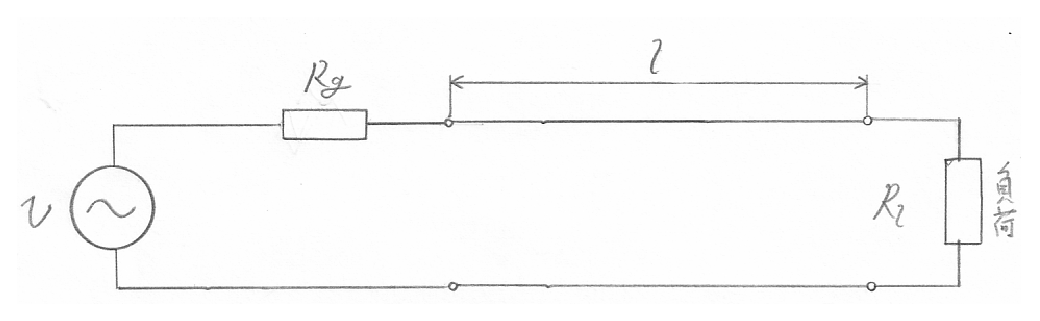
\includegraphics[width=0.4\textwidth]{IMG_20250410_0001.eps}
  \caption{電気信号の伝達}
  \label{a}
\end{figure}

低周波で信号を伝えた場合、電圧・電流は受信点に瞬時に伝達すると考えて問題ないが、周波数が高くなると受信点の負荷$R_1$に正の信号が伝達する前に信号源が
負の信号を出すという事態が発生する。この事態を取り扱うために、低周波での交流理論を拡張する方法と導体に沿って伝達される電磁波として取り扱う
方法がある。

\subsection{伝送線路方式}

伝送線路を詳しく調べると、導体に起因するインダクタンス$\Delta L$とキャパシタンス$\Delta C$が一様に分布していて図\ref{b}のように表すことができる。

\begin{figure}[H]
  \centering
  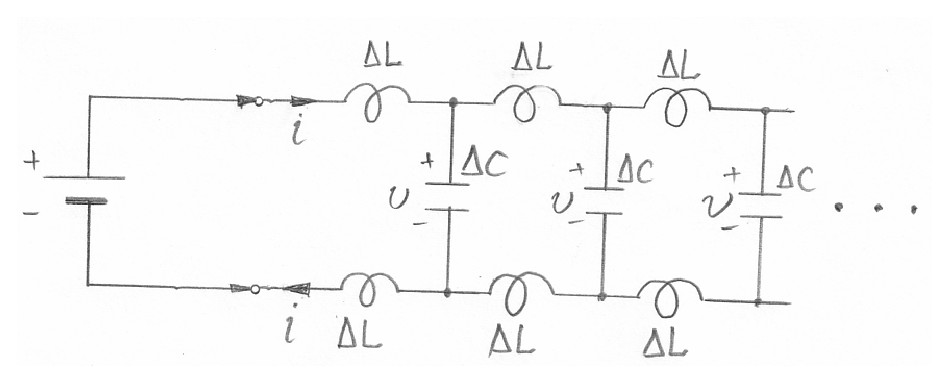
\includegraphics[width=0.4\textwidth]{IMG_20250410_0002.eps}
  \caption{分布定数線路}
  \label{b}
\end{figure}

また、導体の単位長あたりの損失抵抗$R$と損失コンダクタンス$G$を含め、さらに各点における電圧、電流を考えると、図\ref{c}のようになる。

\begin{figure}[H]
  \centering
  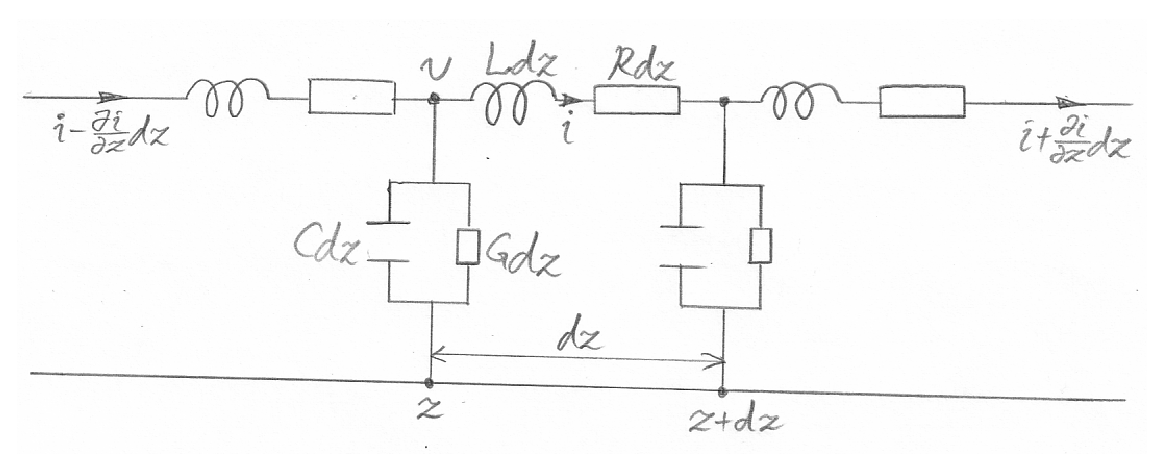
\includegraphics[width=0.4\textwidth]{IMG_20250410_0003.eps}
  \caption{分布定数線路の区間$dz$での等価回路}
  \label{c}
\end{figure}

この回路をキルヒホッフの法則を用いて立式し、得た数式を変形すれば以下のよう\textbf{分布定数回路の微分方程式(telegrapher's equiations)}を得る。

\begin{align}
  -\frac{\partial v}{\partial z}=L\frac{\partial i}{\partial t}+Ri \\
  -\frac{\partial i}{\partial z}=C\frac{\partial v}{\partial t}+Gv
\end{align}

\subsection{波動方程式}

図\ref{c}の回路において損失$R,G$がない場合を考える。式(1),(2)に対して$R=0,G=0$を代入し、もう一度偏微分して二階の偏微分方程式を
つくったあと$i,v$のどちらかを消去すれば、\textbf{無損失線路の波動方程式}を得る。



\begin{align}
  \frac{\partial^2 v}{\partial z^2}=LC\frac{\partial^2 v}{\partial t^2}
\end{align}

上式は$i$を消去したため電圧に関する式となっている。

波動方程式に関してはダランベールの解が得ることが知られており、式(3)では

\begin{align}
  v(z.t)=v_1(v_pt-z)+v_2(v_pt+z)
\end{align}

を得る。視覚上の注意として、$v_1,v_2$は()に対して掛け算をしているわけではなく関数$f(x)$の()と同じ意味の括弧である。

この解を式(3)に代入すると、

\begin{align}
v_p=\frac{1}{\sqrt{LC}}
\end{align}

を得る。

ここで、第一項$v_1(v_pt-z)$に注目し、以下のように特徴を浮かび上がらせてみる。

\begin{enumerate}
\item $v_1(v_pt-z)$のどこか一点に着目すると、$v_pt-z=\mathrm{const.}$と表せる。わかりにくいので例として適当な関数$f(x)$において$x$を決定してみる。すると$f(x)$は決定され特定の値を持つ。即ち逆に言えば、$f(x)$の曲線上のどこか一点を見つめれば、$x$は決定していることになる。これを$x=\mathrm{const.}$と書き、一定という意味である。
\item 式変形すれば、$z=v_pt-\mathrm{const.}$となる。
\item 左辺にある変数は$t$のみなので、位置$z$は$t$の関数$z(t)$であるということがわかる。
\item 古典力学で位置を特定するには、$x(t)=v_0t+\frac{1}{2}at^2$であり、これにのっとると$z(t)=v_pt-\mathrm{const.}$では、波形がz軸正方向に速度$v_p$で進んでいる事がわかる。
\end{enumerate}

以上のことを図に表現すると、図\ref{d}のように表せる。

\begin{figure}[H]
  \centering
  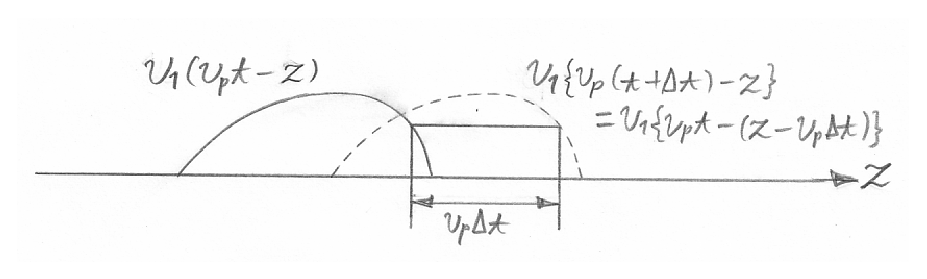
\includegraphics[width=0.4\textwidth]{IMG_20250410_0004.eps}
  \caption{電圧進行波}
  \label{d}
\end{figure}


また、このことは第二項$v_2(v_pt+z)$にも同様に適応でき、その場合波形はz軸の負方向にすすむ。

今回は電圧$v$で示したが、式(4)を電流に関して得ることにより、電流波形に関しても上記と同様のことが言える。

\subsection{正弦波動}

基本的な波形である正弦波の伝搬に関して考える。まず電圧$v$と電流$i$を0とした無損失の場合を考える

\begin{align}
  v=\sqrt{2}Ve^{j\omega t},i=\sqrt{2}Ie^{j\omega t}
\end{align}

とする。ここで$V,I$は複素振幅であり、$z$に関する関数のため$t$には依存していない。

これらを分布定数回路の微分方程式(1),(2)に代入すると、

\begin{align}
  -\frac{dV}{dz}=(R+j\omega L)I\\
  -\frac{dI}{dz}=(G+j\omega C)V
  \end{align}

を得る。(7)を$z$で偏微分し(8)を代入すると$I$が消去され

\begin{align}
  \frac{d^2 V}{dz^2}=(R+j\omega L)(G+j\omega C)V
  \end{align}

という線形微分方程式を得る。なので$e^{\lambda z}$という形の解を仮定して$V$に代入すると

\begin{align}
  \lambda ^2=(R+j\omega L)(G+j\omega C)
  \end{align}

という特性方程式を得る。ただし、$R,G$は$\omega L,\omega C$に対し十分小さいとする。ここで$\gamma = \alpha +j\beta(\lambda = \pm \gamma)$とおくと、

\begin{align}
  \alpha = \frac{R\sqrt{C/L}+G\sqrt{L/C}}{2}, \beta = \omega \sqrt{LC}
  \end{align}

となり、これを用いて式(9)は

\begin{align}
  V=Ae^{-\gamma z}+Be^{\gamma z}
\end{align}

と表現できる。ここで$A,B$は線路の\textbf{境界条件}により定まる定数である。

電流に関しても同様に、

\begin{align}
  I=A\sqrt{\frac{Y}{Z}}e^{-\gamma z}-B\sqrt{\frac{Y}{Z}}e^{\gamma z}
\end{align}

\subsection{伝搬定数}

$V,I$は$z$に依存する複素振幅であったので、まず電圧$V$のみ式(6)に代入すると、

\begin{align}
  v=\sqrt{2}Ae^{j\omega t-\gamma z}+\sqrt{2}Be^{j\omega t+\gamma z}\\
  =\sqrt{2}Ae^{-\alpha z}e^{j(\omega t-\beta z)}+\sqrt{2}Be^{\alpha z}e^{j(\omega t+\beta z)}
  \end{align}

ここで損失$R,G$を無視すると、$\alpha=0$であるので無視をする。$\beta$に関しては式(11)を用いて求めるが、ここで式(5)にも注意すると、

\begin{align}
  \omega t-\beta z=\beta((\omega / \beta)t-z)\\
  =\beta(1/\sqrt{LC}t-z)=\beta (v_pt-z)\notag
  \end{align}

と書くことができ、この形は式(4)と同じであるため、正弦波電圧は結局$v_p=\omega /\beta=1/\sqrt{LC}$で$z$軸正方向に伝搬していることが分かる。
また、$\beta z$の項は$sin(\omega t+\theta)$の形と比較して$\theta$に当たるため、$z$おける位相を表しているとわかる。そのため$\beta$は\textbf{位相定数}と呼ばれる。

また、波長$\lambda_g$と$\beta$の間に$\beta \lambda_g=2\pi$の関係が成り立つ。

つぎに損失$R,G$を考慮すると、$e^{-\alpha z}$は$z$に伴って指数関数的に減少していくことがわかる。
そのため$\alpha$を\textbf{減衰定数}とよび、$\gamma =\alpha +j\beta$は\textbf{伝搬定数}と呼ばれる。

上記と同様のことを式(14)の第二項に適応すれば、第二項はz軸負方向に伝搬することがわかり、式(13)の電流に関しても全く同様のことが言える。

\subsection{特性インピーダンス}

電圧の前進波、後進波をそれぞれ$\overrightarrow{V}=Ae^{-\gamma z},\overleftarrow{V}=Be^{\gamma z}$、電流の前進波、後進波をそれぞれ
$\overrightarrow{I}=A\sqrt{Y/Z}e^{-\gamma z},\overleftarrow{I}=B\sqrt{Y/Z}e^{\gamma z}$とおく。このとき
前進波の電圧と電流の比をとると、

\begin{align}
\frac{\overrightarrow{V}}{\overrightarrow{I}}=\frac{Ae^{-\gamma z}}{A\sqrt{Y/Z}e^{-\gamma z}}=\sqrt{\frac{Y}{Z}}\equiv Z_{0}
\end{align}

と、線路により定まる定数のインピーダンスが分かる。このインピーダンス$Z_{0}$を波動インピーダンス、特性インピーダンスと呼ぶ。
この定数は後進波で同じ操作をしても等しい。

続いて、式(7),(8)より、

\begin{align}
R+j\omega L=Z \\
G+j\omega C=Y
\end{align}

とし、式(17)に代入すると、

\begin{align}
Z_{0}=\sqrt{\frac{Z}{Y}}=\sqrt{\frac{L}{C}}\left\{1-j\left(\frac{R}{2\omega L}-\frac{G}{2\omega C}\right) \right\} 
\end{align}

となる。$Z_0$は一般に虚数であるが、基本虚数部分は小さいので

\begin{align}
Z_0=\sqrt{L/C}
\end{align}

と表すことができる。
これは\textbf{純抵抗}と呼び、以下断りのない限り$Z_0$は純抵抗である。

\subsection{前進波}

図\ref{e}に示すような、内部インピーダンス$Z_g$で正弦波の信号$V_g$を出力する信号源があり、かつ線路が$+z$方向に無限に続く線路を考える。
ここで線路の境界条件が定められたことになるので、式(12)、(13)の$A,B$が決定したはずである。

\begin{figure}[H]
  \centering
  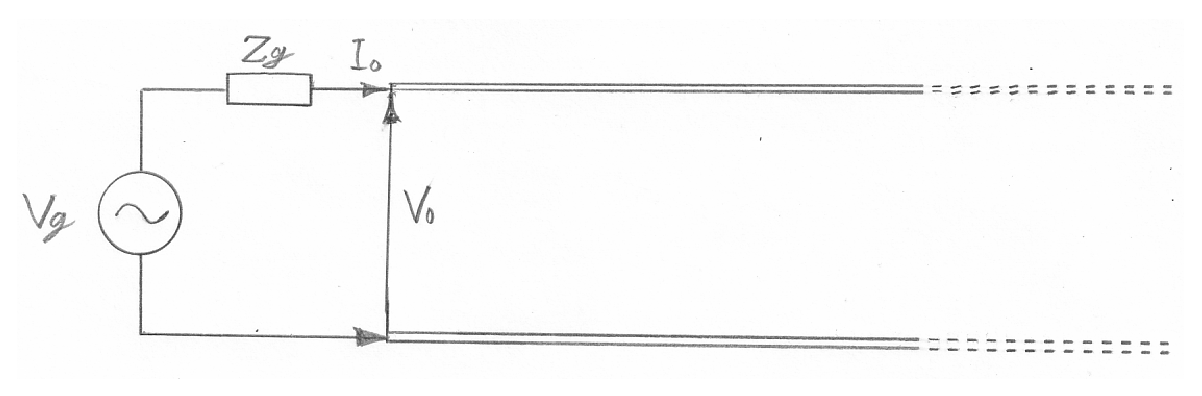
\includegraphics[width=0.4\textwidth]{IMG_20250410_0006.eps}
  \caption{線路}
  \label{e}
\end{figure}

式(12)の$Be^{\gamma z}$は、$z$が$+\infty$になるので、この項は物理的な意味合いを持たない項となる。そのため$B=0$とし、
$z=0$での電圧を$V_0$とすれば、

\begin{align}
V_0=A
\end{align}

を得る。電流に関しても同様に式(15)より

\begin{align}
I_0=A\sqrt{Y/Z}=A/Z_0
\end{align}

電圧、電流よりインピーダンスを求めると、

\begin{align}
\frac{V_0}{I_0}=\sqrt{\frac{Z}{Y}}=Z_0
\end{align}

つまり、無限長の線路では、入力インピーダンスは特性インピーダンスと等しい。
そのため、等価回路として図\ref{f}が描ける。

\begin{figure}[H]
  \centering
  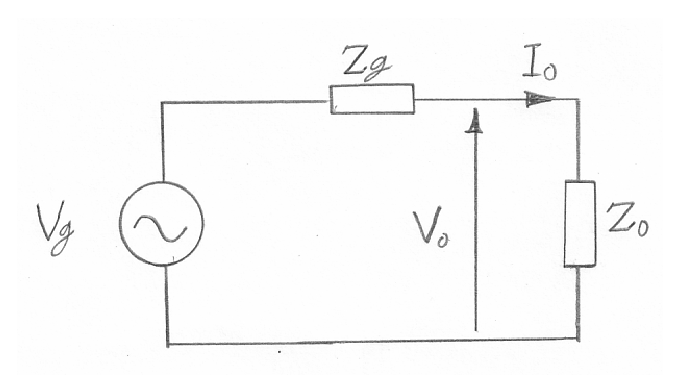
\includegraphics[width=0.4\textwidth]{IMG_20250410_0007.eps}
  \caption{等価回路}
  \label{f}
\end{figure}

図\ref{e}の$V_g$はキルヒホッフの法則より

\begin{align}
V_g=Z_gI_{0}+V_0
\end{align}

式(22)、(23)、(25)より$V_0,I_0$を消去すれば、

\begin{align}
A=V_g/\left(  1+Z_g/Z_0 \right)
\end{align}

となり、積分定数$A$を得ることができる。これを式(12)に代入し、電圧は

\begin{align}
V=\overrightarrow{V}\frac{Z_0V_g}{Z_0+Z_g}e^{-\left(   \alpha +j\beta\right)z}
\end{align}

であることがわかり、同様に電流は式(13)より

\begin{align}
I=\overrightarrow{I}=\frac{V_g}{Z_0+Z_g}e^{-\left(   \alpha +j\beta\right)z}
\end{align}

続いて、電圧と電流の複素共役との積における実部をとると、線路に伝搬する電力$P$を得る。

\begin{align}
  P=\mathrm{Re}VI^*=\left\lvert \frac{V_g}{Z_0+Z_g}\right\rvert ^2\mathrm{Re}Z_0\cdot e^{-2\alpha z}\\
  =\frac{\left\lvert V_g\right\rvert^2 }{4\mathrm{Re}Z_g}\cdot \frac{4\mathrm{Re}Z_g\cdot\mathrm{Re}Z_0}{\left\lvert Z_g+Z_0\right\rvert }\cdot e^{-2\alpha z}
  \end{align}

  この式は以下のように解釈できる。

  \begin{enumerate}
  \item $\left\lvert V_g\right\rvert ^2/4\mathrm{Re}Z_g$は信号源の固有電力(最大電力)である。
  \item 固有電力が式中央の係数$4\mathrm{Re}Z_g\cdot \mathrm{Re}Z_0/\left\lvert Z_g+Z_0\right\rvert^2 \leq 1$だけ割りさかれ、伝送線へと伝わる。
  \item 共役整合の条件$Z_g^*=Z_0$を電源と線路とが満たしたときは、式中央の係数が1となり、固有電力はすべて割さかれずに線路に流入する。
  \item 最後の係数$e^{-2\alpha z}$を見ると、電力が伝搬するに伴って指数関数的に減少していくことがわかる。
  \end{enumerate}
  
  また、4.の$\alpha$は式(20)より損失$R,G$に基づくものとわかる。これはつまり、線路を伝搬する途中に熱としてエネルギーが失われていくことを示している。
  
  
\subsection{反射波}


図\ref{g}に示すような、伝送線路を考える。この線路は図\ref{e}で示した無限長の線路に対して、長さを$l$とし、負荷$Z_l$を追加したものである。
$z=0$の電圧を$V_0,I_0$とすると、式(21),(22)は以下のようになる。

\begin{figure}[H]
  \centering
  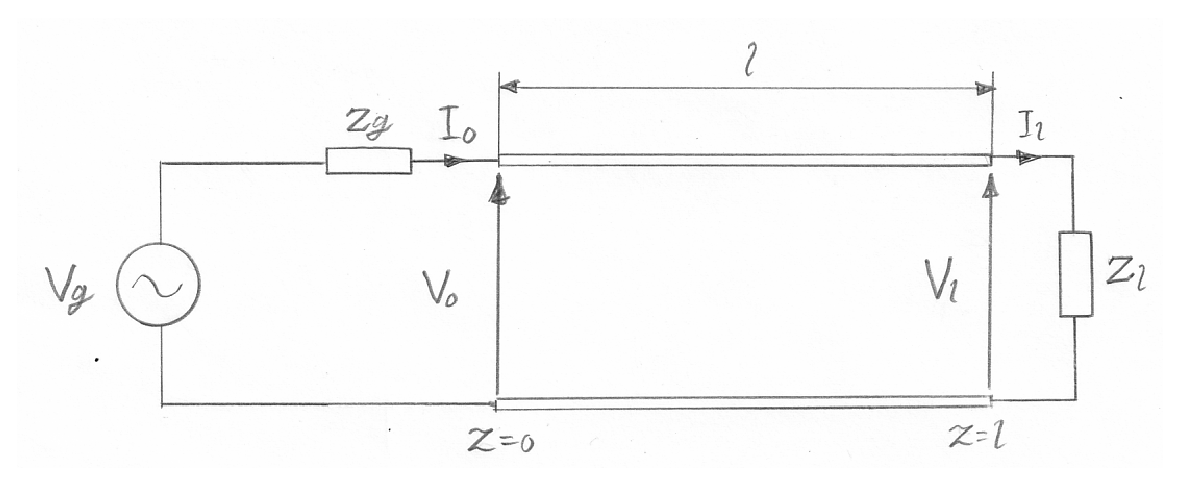
\includegraphics[width=0.4\textwidth]{IMG_20250410_0009.eps}
  \caption{線路による信号の伝達}
  \label{g}
\end{figure}

\begin{align}
V_0=A+B,I_0=A/Z_0-B/Z_0
\end{align}

そして、次に$z=l$での電圧、電流を同じように$V_l,I_l$とすると、

\begin{align}
V_l=Ae^{-\gamma l}+Be^{\gamma l},I_l=Ae^{-\gamma l}/Z_0-Be^{\gamma l}/Z_0
\end{align}

である。ここで信号源、負荷端子にキルヒホッフの法則を適応し、

\begin{align}
V_g=Z_g+V_0,V_l=Z_lI_l
\end{align}

となる。
ここで、特性インピーダンス$Z_0$を実数とし、整合条件$Z_g=Z_0$をみたしているとすると、式(43),(44),(45)より

\begin{align}
A=\frac{V_g}{2}, B=\frac{V_g}{2}\cdot \frac{Z_l-Z_0}{Z_l+Z_0}e^{-2\gamma l}
\end{align}

を得る。

これを電圧式(21)、電流の式(22)にあてはめると、

\begin{align}
V=\frac{V_g}{2}e^{-\gamma z}+\frac{V_g}{2}e^{-\gamma l}\cdot \frac{Z_l-Z_0}{Z_l+Z_0}e^{-2\gamma (l-z)} \\
I=\frac{V_g}{2Z_0}e^{-\gamma z}-\frac{V_g}{2Z_0}e^{-\gamma l}\cdot \frac{Z_l-Z_0}{Z_l+Z_0}e^{-2\gamma (l-z)}
\end{align}

この結果について解釈すると以下のようになる。

\begin{enumerate}
\item 第一項は前進波であり、その振幅$A$は$V_g$の半分である。
\item 第二項は後進波であり、この波は負荷$Z_l$により第一項の波が反射して生じたために発生した。
\item 前進波は$z=l$に辿り着くまでに位相は$\gamma l$だけ遅れている。
\item $Z_l$において前進波は一部消費され、$\varGamma _l=\frac{Z_l-Z_0}{Z_l+Z_0},\left\lvert \varGamma _1\right\rvert <1$の分は反射され、電源へ戻る。
\item $z=l$から$z=z$へ戻るまでに位相はさらに$\gamma \left(  l-z \right)$遅れる。
\end{enumerate}

ここで登場した$\varGamma _1$は$z=l$における\textbf{電圧反射係数}と呼ばれている。整合条件$Z_l=Z_0$であれば、$\varGamma=0$となる。

\subsection{定在波}

前進波(入射波)とそれにより生じた後進波(反射波)が存在する場合、任意の点$z$における電圧は

\begin{align}
V=\overrightarrow{V}+\overleftarrow{V}=Ae^{-\gamma z}+Be^{\gamma z}
\end{align}

であり、前進波は大抵後進波より大きいので

\begin{align}
A=A'+B^*
\end{align}

とおき、$\alpha =0,\gamma = j/beta$の無損失の場合を考えると式(37)は

\begin{align}
V=A'e^{-j\beta z}+B^*e^{j\beta z}+Be^{j\beta z} \\
=A'e^{j\beta z}+2\left\lvert B\right\rvert \cos \left(   \beta z+\phi '\right) \notag
\end{align}

と書くことができ、$B=\left\lvert B\right\rvert e^{j\phi '} $である。この式の第一項はz軸正方向に移動するが、第二項は
前進波の一部$B=\left\lvert B\right\rvert e^{j\beta z}$と後進波(反射波)$Be^{j¥beta z}$が干渉し、z軸のどちらにも進まない波ができる。
この移動しない波を\textbf{定在波}という。

\subsection{反射係数}

電圧に関する前進波と後進波の比を

\begin{align}
\varGamma \equiv \left\lvert \varGamma \right\rvert e^{j\theta} \\
=\frac{\overleftarrow{V}}{\overrightarrow{V}}=\frac{Be^{j\beta z}}{Ae^{-j\beta z}}=\frac{B}{A}^{j2\beta z}=\left\lvert \frac{B}{A}\right\rvert e^{j\left(   2\beta z +\phi\right)} \notag
\end{align}

とおいたとき、$\varGamma$は任意の点$z$の\textbf{電圧反射係数}という。

\begin{align}
\theta = 2\beta z+\phi,B/A=\left\lvert B/A\right\rvert e^{j\phi}
\end{align}

であり、$\left\lvert \varGamma \right\rvert =\left\lvert B/A\right\rvert \leq 1$となっている。
$\varGamma$は一定であり、$z$の変化により角度$\theta$が変化するので、図示をすれば図\ref{h}のようになる。

\begin{figure}[H]
  \centering
  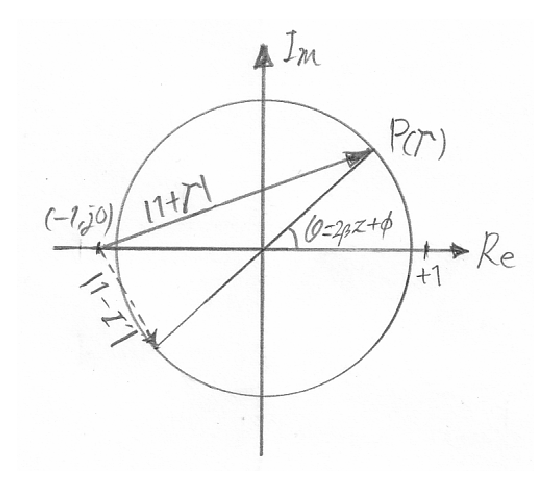
\includegraphics[width=0.4\textwidth]{IMG_20250410_0010.eps}
  \caption{反射係数平面}
  \label{h}
\end{figure}

この図は\textbf{クランク図}と呼ばれる。

式(40)を式(37)に代入すると

\begin{align}
  \left\lvert V\right\rvert =\left\lvert Ae^{^j\beta z}+\varGamma Ae^{-j/beta z}\right\rvert = \left\lvert A\right\rvert \cdot\left\lvert 1+\varGamma\right\rvert 
  \end{align}

を得て、図\ref{h}で
$\left(   -1,j\theta \right)$と$P(\varGamma)$を結ぶ線の線分$\left\lvert 1+\varGamma\right\rvert $
を求めプロットすることにより、電圧定在波
を得ることができる。

電流も電圧と同じように導出すれば、

\begin{align}
\left\lvert I\right\rvert =\frac{1}{Z_0}\cdot \left\lvert A\right\rvert \cdot\left\lvert 1-\varGamma\right\rvert 
\end{align}

に、図\ref{h}で求めた$\left\lvert 1+\varGamma\right\rvert $をプロットすれば、電流定在波が得られる。

\subsection{定在波分布}

図\ref{g}における定在波を調べる。負荷$z=l$の電圧反射係数を

\begin{align}
  \varGamma_l\equiv\left|\varGamma _l\right|e^{j\theta _l}=\left|\frac{B}{A}\right|e^{j\left(2\beta l+\phi\right)}=\frac{Z_l-Z_0}{Z_l+Z_0}
  \end{align}
  
  とおくと、任意の点$z$における反射係数と、$z=l$の反射係数$\varGamma _l$を関連付ける式
  
  \begin{align}
  \varGamma=\varGamma _le^{j2\beta\left(z-l\right)},\left|\varGamma\right|=\left|\varGamma _l\right|
  \end{align}
  
  を得る。これを式(42)に代入し
  
  \begin{align}
  \left|V\right|=\left|A\right|\cdot\left|1+\varGamma _le^{j2\beta\left(z-l\right)}\right|
  \end{align}
  
  となる。この式を図にすると図\ref{i}のようになる。この波の最大値は$1+\left|\varGamma _l\right|=1+\left|\varGamma\right|$であり、最小値は
  $1-\left|\varGamma _l\right|=1-\left|\varGamma\right|$
  である。

  \begin{figure}[H]
    \centering
    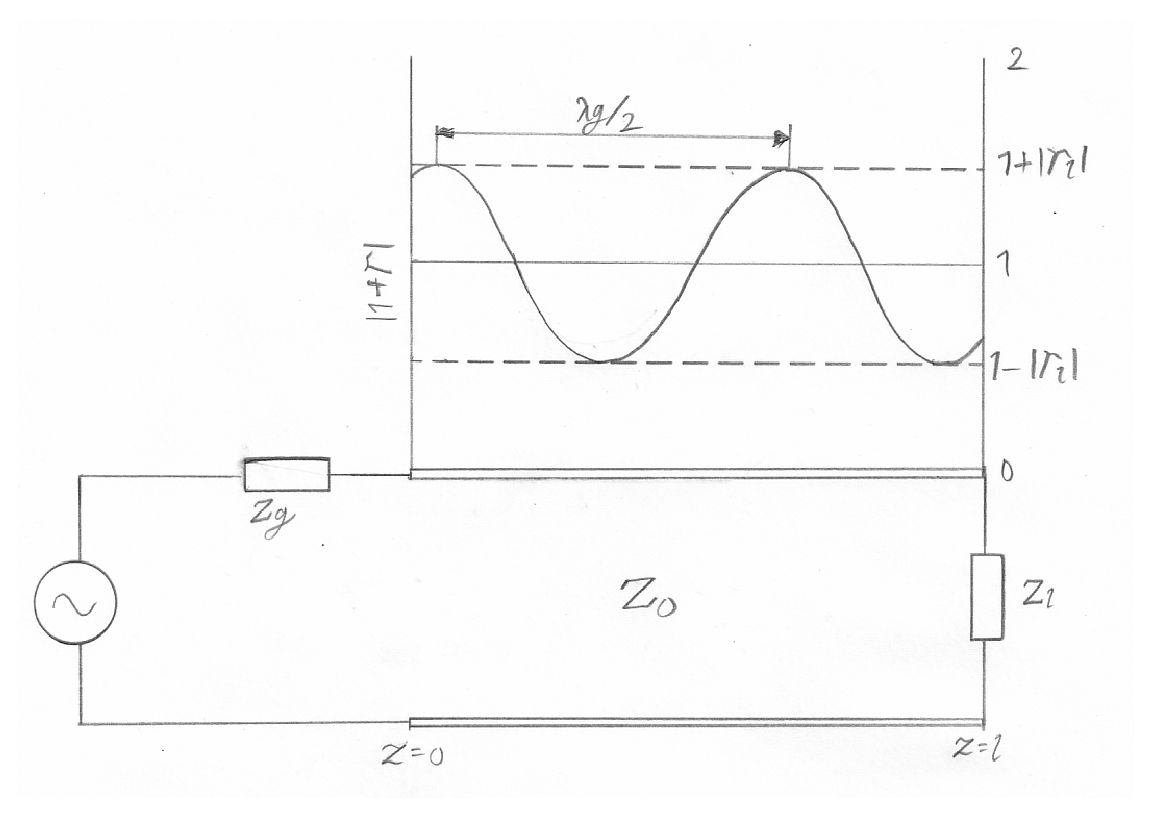
\includegraphics[width=0.5\textwidth]{IMG_20250410_0011.eps}
    \caption{電圧定在波分布}
    \label{i}
  \end{figure}
  
  また、$\varGamma$の周期$\Delta z$は$2\beta\Delta z=2\pi$であるので、
  
  \begin{align}
  \Delta z=\frac{\pi}{\beta}=\frac{\lambda _g}{2}
  \end{align}
  
  が成り立つので、定在波の山谷の感覚は半波長となっている。
  
  
  \subsection{定在波比}
  
  反射係数$\varGamma _l$により生じる電圧定在波の最大値$\left|V\right|_\mathrm{max}$、最小値$\left|V\right|_\mathrm{min}$で比をとると、電圧に関する\textbf{定在波比}である$\rho$を得る。
  
  \begin{align}
  \rho=\frac{\left|V\right|_\mathrm{max}}{\left|V\right|_\mathrm{min}}=\frac{1+\left|\varGamma _l\right|}{1-\varGamma _l}=\frac{1+\left|\varGamma\right|}{1-\varGamma}
  \end{align}
  
  $\left|\varGamma\right|$についてとく
  
  \begin{align}
  \left|\varGamma _l\right|=\left|\varGamma\right|=\frac{\rho-1}{\rho+1}
  \end{align}
  
  定常波の最小点が負荷端から信号源側へ$d_m$の位置にあるすると、式(47)に$z=l-d_m$を代入し
  
  \begin{align}
  \left|V\right|\mathrm{min}|/\left|A\right|\equiv 1-\left|\varGamma _l\right|=\left|1+\varGamma _le^{-j2\beta d_m}\right|
  \end{align}
  
  なので、負荷端の反射係数の位相角は
  
  \begin{align}
  \theta _l=2\beta d_m+\left(2n+1\right)\pi,n\in \mathbb{Z}
  \end{align}
  
  となる。
  つまり、$\rho$及び$d_m$が分かれば、$\left|\varGamma _l\right|=\left|\varGamma\right|$と$\theta_l$が求まる。
  
  以上のことは電流の定在波に関しても同じであるが、反射係数が逆の符号となり、電流の定在波は電圧の定在波を$\lambda _g/4$ずらしたもじょである。
  
  \subsection{インピーダンス測定}
  
  式(44)を
  
  \begin{align}
  Z_l=Z_0\frac{1+\varGamma _l}{1-\varGamma _l}
  \end{align}
  
  と、変形すれば、負荷インピーダンス$Z_l$が求められる。この式に式(49)、(51)を用いて以下のように変形する
  
  \begin{align}
  \frac{Z_l}{Z_0}=\frac{\cos\beta d_m-j\rho \sin\beta d_m}{\rho\cos\beta d_m-j\sin\beta d_m}
  \end{align}
  
  であるので、これは$\rho$と$d_m$より$Z_l$が求まることを示している。
  
  \subsection{線路上のインピーダンス}
  
  $Z_l$が定まったことにより
  式(45)を用いて任意の点$z$における反射係数$\varGamma$を知ることができる。$z$から負荷側をみたインピーダンスを$Z$としたとき、この点に$Z$の負荷が繋がっているとみなせるばそうすると、式(1.45)の$Z_l$を$Z$、$\varGamma _l$を$\varGamma$とすれば
  
  \begin{align}
  \varGamma=\frac{Z-Z_0}{Z+Z_0}
  \end{align}
  
  を得る。この式を$Z$についてとき式(1.46)、(1.45)を用いると
  
  \begin{align}
  Z=Z_0\frac{Z_l-jZ_0\tan\beta\left(z-l\right)}{Z_0-jZ_l\tan\beta\left(z-l\right)}
  \end{align}
  
  と、$Z$が求まる。$Z_l=Z_0$である時は、$Z=Z_0$がなりたつ。 
  $z$と負荷の距離を

  \begin{align}
  d=l-z
  \end{align}

とし、$Z,Z_l$を$Z_0$で\textbf{規格化}したものを

\begin{align}
\hat{Z}=Z/Z_0,\hat{Z_l}=Z_l/Z_0
\end{align}

とすれば、式(55)は

\begin{align}
\hat{Z}=\frac{\hat{Z_l}+j\tan\beta d}{1+j\hat{Z}\tan\beta d}
\end{align}

と、簡略化することができる。

以上をもって、分布定数回路の基本的な概念の説明は終える。

\section{マクスウェル方程式}

図\ref{b}のような伝送線路を仮定したとき、単位量あたりのインダクタンスとキャパシタンスを考慮した。
インダクタンスができたのは、導体の周囲に磁界が生じたことによってであり、またキャパシタンスができたのは
導体間に電界が生じたということによってである。
これは即ち、電気信号が導体に沿って進めばそれに伴った磁界と電界が線路に伝搬するということである。

ここからはマクスウェル方程式を用いて、電磁界による三次元空間のことを取り扱っていく。これは位置次元で考えていた
伝送線路よりもより複雑で、より根本的である。

そもそもマクスウェル方程式とは、ファラデーの電磁誘導、アンペールの回路法則、電磁波に関するガウスの定理を簡潔な方程式にまとめた
ものであり、まずはこれを導出していく。

\subsection{ガウスの定理(電界)}

電荷$q_1,q_2$が$r$離れて存在するとき、

\begin{align}
F=\frac{q_1 q_2}{4\pi \epsilon r^2}
\end{align}

の力がそれぞれの電荷に加わる。これを電界の式に直すと

\begin{align}
E_1=\frac{1}{\epsilon}\cdot \frac{q_1}{4\pi r^2}
\end{align}

と表せる。$q_2$はこの電界を受けて力が加わったとも言える。$4\pi r^2$に注目すると、力の原因は$q_1$から放射状に出ていることもわかる。

図\ref{j}のように、微小面積$dS$を電界$E$が貫いているとき、$dS$の$E$方向分と$\left\lvert E\right\rvert=E$の積を電力束と定義すると、電力束は

\begin{figure}[H]
  \centering
  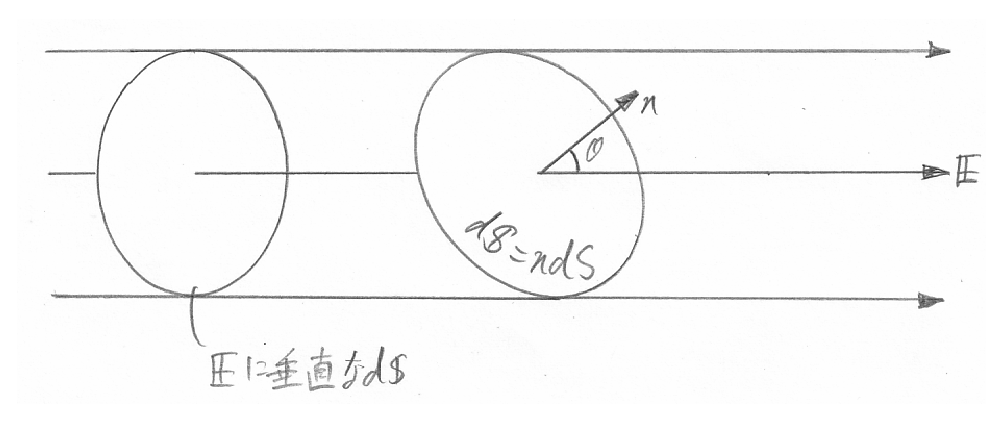
\includegraphics[width=0.4\textwidth]{IMG_20250410_0012.eps}
  \caption{電力束}
  \label{j}
\end{figure}


\begin{align}
dN=dScos\theta \cdot E = E\cdot dS
\end{align}

と表せる。この定義から式(61)の$q_1$からでるすべての電力束を求めると、

\begin{align}
N=\int E\cdot dS=E_1\cdot 4\pi r^2=\frac{q_1}{\epsilon}
\end{align}

となる。この式からわかるように、電力束は誘電率$\epsilon$により変化してしまうので、電束$D=\epsilon E$を定義する。すると

\begin{align}
\int D\cdot dS=\epsilon E_1\cdot 4\pi r^2=q_1
\end{align}

と表せる。この式より、電束は電荷によってのみ量が変化することがわかる。

次に図\ref{k}に示すような体積$V$の中に電荷が密度$\rho$で分布しているとする。この体積の表面から出る電束は内部の電荷の総量に等しく、

\begin{figure}[H]
  \centering
  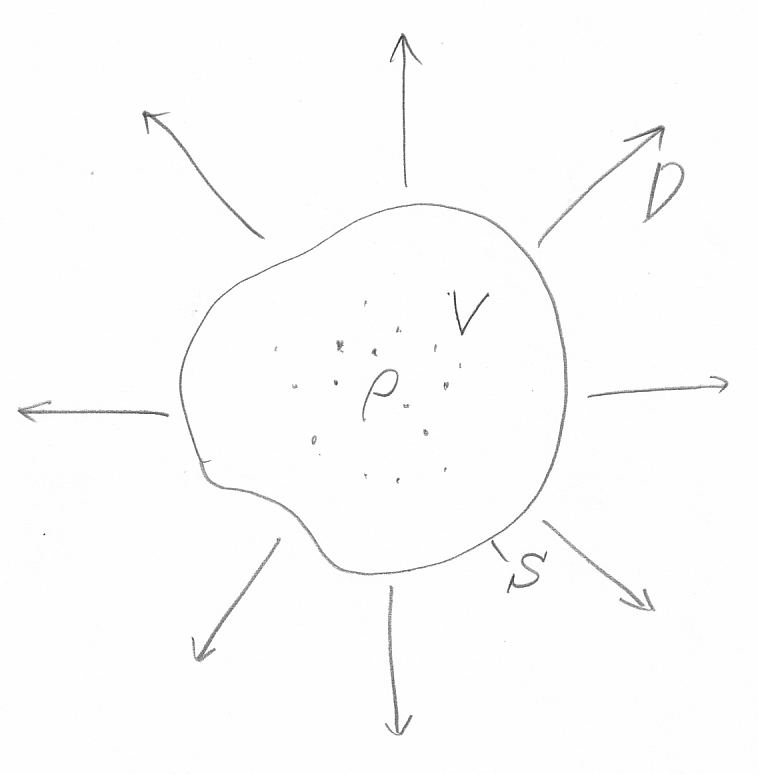
\includegraphics[width=0.4\textwidth]{IMG_20250411_0001.png}
  \caption{体積$V$内の電荷分布}
  \label{k}
\end{figure}

\begin{align}
\int_{S} D\cdot dS=\int_{V}\rho dV
\end{align}

である。また、体積の外部に電荷があった場合、それから出る電束は体積に入ったあと必ず出るので、この式には影響を及ぼさない。

続いて図\ref{}のような微小体積の箱を考える。
まず、箱の中にある電荷が発生させる電束が$dx$に垂直な2つの面積$dydz$を$dV$の外側に向けて貫く場合を考える。

\begin{figure}[H]
  \centering
  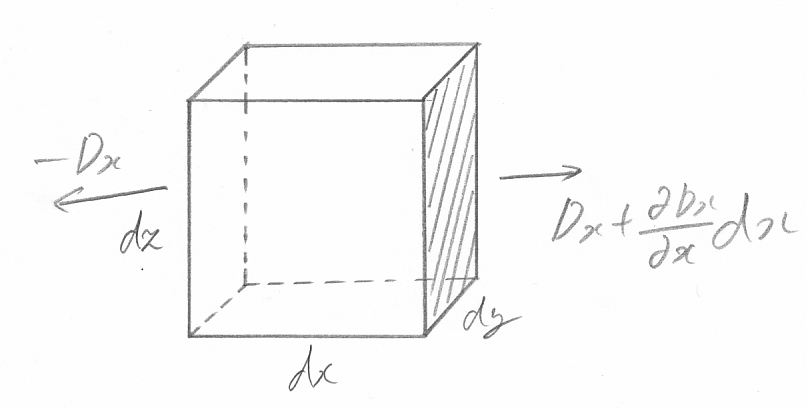
\includegraphics[width=0.4\textwidth]{IMG_20250411_0002.png}
  \caption{微小体積}
  \label{l}
\end{figure}

\begin{align}
-D_xdydz+(D_x+\frac{\partial D_z}{\partial x}dx)dydz=\frac{\partial D_x}{\partial x}dxdydz=\frac{\partial D_x}{\partial x}dV
\end{align}

同様に他の面から出る電束は

\begin{align}
\frac{\partial D_y}{\partial y}dV\\
\frac{\partial D_z}{\partial z}dV
\end{align}

であり、この直方体から出る全ての電束は和で与えることができ、

\begin{align}
\left( \frac{\partial D_x}{\partial x}+\frac{\partial D_y}{\partial y}+\frac{\partial D_z}{\partial z} \right)dV=\rho dV
\end{align}

この式は体積$dV$よし出る電束を表すので、( )の中をベクトル$\bm{D}$の発散と呼び

\begin{align}
\mathrm{div} \bm{D}\equiv \frac{\partial D_x}{\partial x}+\frac{\partial D_y}{\partial y}+\frac{\partial D_z}{\partial z}
\end{align}

と表現でき、式(65)を$dv$で割ることで

\begin{align}
\mathrm{div}\bm{D}=\rho
\end{align}

と書き表せる。これは\textbf{電界に関するガウスの定理}であり、式(64)の微分形式である。式(68)を体積$V$で積分したものは
式(64)と等しいので、

\begin{align}
\int _SD\cdot dS=\int _V\mathrm{div}DdV
\end{align}

これはベクトル$\bm{D}$の表面積分を体積積分に変換する公式であり、これもまたガウスの定理と呼ばれる。

ここで三次元空間$x,y,z$のそれぞれの方向に伸びる単位ベクトル$i,j,k$を用いて、
\begin{align}
\nabla\equiv i\frac{\partial}{\partial x}+j\frac{\partial}{\partial y}+k\frac{\partial}{\partial z}
\end{align}

とあらわされる演算記号$\nabla$を導入し、式(69)を

\begin{align}
\mathrm{div}\bm{D}=\nabla\cdot \bm{D}
\end{align}

と表す。

\subsection{ガウスの定理(磁界)}

電界に関するガウスの定理について述べたものを流用するために、表\ref{m}のように電界と磁界に関する諸性質を対応させる。

\begin{table}[H]
\centering
\caption{電気量と磁気量}
\begin{tabular}{c|c}
  \hline
  電荷$q$ & 磁荷$m$ \\
  \hline
  電界$\bm{E$} & 磁界$\bm{H}$\\
  誘電率$\epsilon$ & 透磁率$\mu$\\
  電束密度$\bm{D}$ & 磁束密度$\bm{B}$\\
  \hline
\end{tabular}
\label{m}
\end{table}

しかし、磁界には電界と相違点がひとつある。電界では、電荷は+、-として単独での存在が許されたが、磁界では正の磁荷があるなら必ず同時に負の磁荷が
必ず存在し、逆もまたその然りなのである。このように絶対に二対で存在し、これらを磁気双極子と呼ぶ。

従って図\ref{k}のような状況を用意したとき、磁束は必ず中に戻りその総数は0となる。よって

\begin{align}
\mathrm{div}\bm{B}=0
\end{align}

となっている。

\subsection{アンペールの回路則}

コイルを作成し電流を流せば、図\ref{n}のような電磁石になる。

\begin{figure}[H]
  \centering
  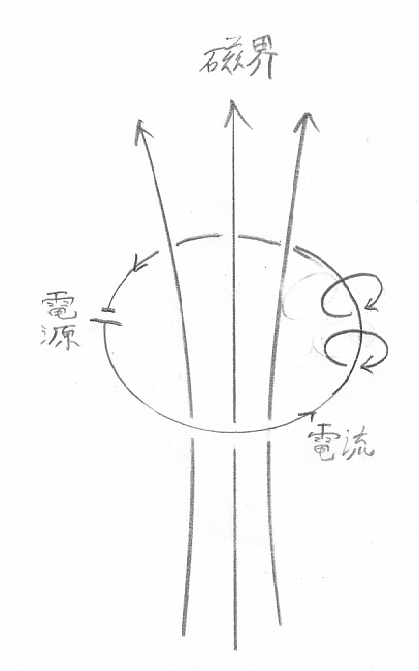
\includegraphics[width=0.25\textwidth]{IMG_20250411_0003.png}
  \caption{電磁石}
  \label{n}
\end{figure}

電流がある方向から流れるとそれを囲むように磁界$\bm{H}$が発生する。なので
図\ref{n}では、そのように発生した磁界$\bm{H}$が円状にとりまくのでコイルを貫く磁束が生じたのである。

図\ref{o}において、半径$r$、長さ$dl$で電流を囲む微小円筒を考える。磁界$\bm{H}$は電流$\bm{I}$から放射状に
広がると考えると、$r$での磁界$\left|\bm{H}\right|$を円筒表面$2\pi r\cdot dl$で積分したものが$dl$の電流
$\bm{I}$に比例すると推察できる。この比例は、MKSA単位系で1となり

\begin{figure}[H]
  \centering
  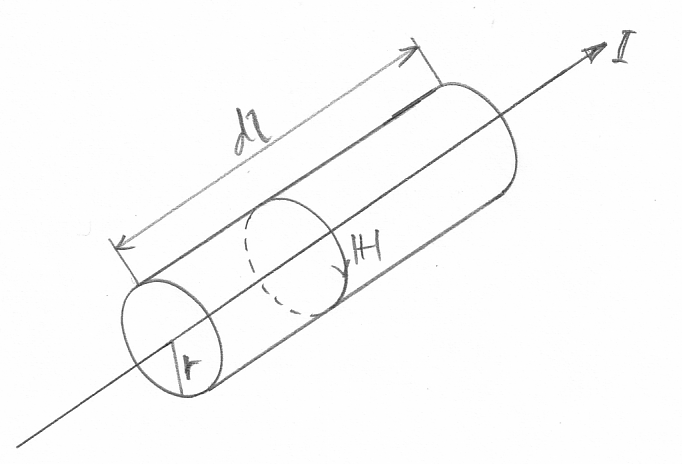
\includegraphics[width=0.4\textwidth]{IMG_20250411_0004.png}
  \caption{電流の磁気作用}
  \label{o}
\end{figure}

\begin{align}
\left|\bm{H}\right|\cdot 2\pi r\cdot dl=\left|\bm{I}\right|\cdot dl
\end{align}

である。この式は半径$r$の大きさに無関係に成立するはずであるから、図\ref{p}にしめすように、逆に電流$\bm{I}$を取り囲む任意の半径$r$での閉曲線
$C$と、微小線分
$dS$、磁界$\bm{H}$をとれば、同様の結果を得るはずである。

\begin{figure}[H]
  \centering
  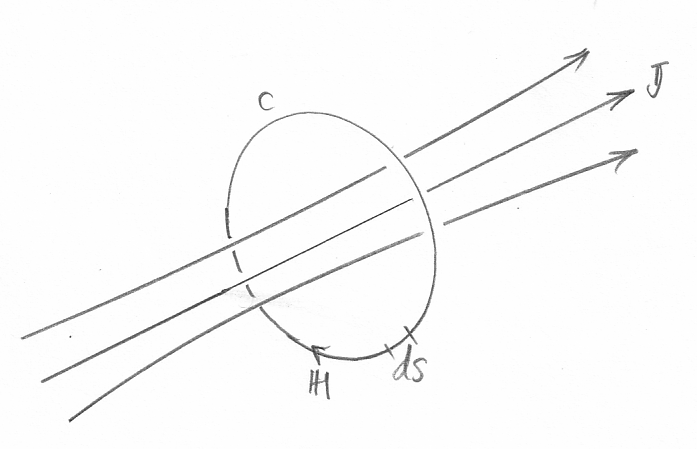
\includegraphics[width=0.4\textwidth]{IMG_20250411_0005.png}
  \caption{電流を囲む任意の閉曲線}
  \label{p}
\end{figure}

ここで電流$\bm{I}$を、閉曲線内に電流密度$\bm{J}$で分布しているとすると、単位長あたりの式

\begin{align}
\oint _C \bm{H}\cdot ds=\int_S\bm{J}\cdot d\bm{S}
\end{align}

と、一般化することができる。これを\textbf{アンペールの回路則}と呼ぶ。ただしここで小文字$s$と大文字$S$は異なるものであり、
$ds$は$C$の微小線分、$S$は$C$に囲まれた面積、$d\bm{S}$は$S$の微小面積ベクトルである。

また、このような閉曲線を考えるときに、閉曲線外部に存在する電流の影響は受けることはない。

つづいて式(76)の微分形を求める。図\ref{q}を考えたとき、面分$d\bm{S}$を貫く電流は

\begin{figure}[H]
  \centering
  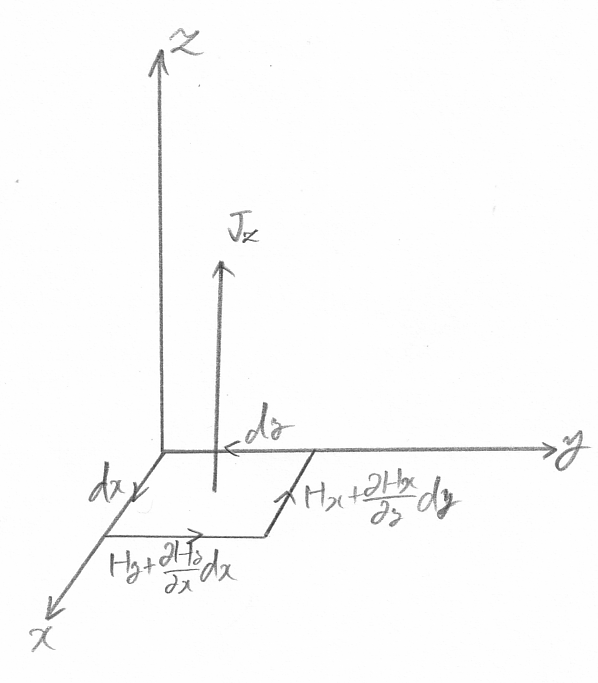
\includegraphics[width=0.4\textwidth]{IMG_20250411_0006.png}
  \caption{面分$dS_z=dxdy$と周辺積分}
  \label{q}
\end{figure}

\begin{align}
\bm{J}\cdot d\bm{S}=J_xdS_x+j_ydS_y+J_zdS_z
\end{align}

であり、次に$J_zdS_z=J_zdxdy$の寄与を求める。

\begin{align}
& J_zdS_z \notag\\
& =H_zdx+\left(H_y+\frac{\partial H_y}{\partial x}dx\right)dy+\left(H_x+\frac{\partial H_x}{\partial y}\right)(-dx)+H_y(-dy)\notag\\
& =\left(\partial{H_y}{\partial x}-\frac{\partial H_x}{\partial y}\right)dS_z
\end{align}

他の成分に関しても同様に求め、ベクトル形式で書くと

\begin{align}
& iJ_x+jJ_y+kJ_z \notag \\
& =i\left(\frac{\partial H_z}{\partial y}-\frac{\partial H_y}{\partial z}\right)+j\left(\frac{\partial H_x}{\partial z}-\frac{\partial H_z}{\partial x}\right) \notag\\
& +k\left(\frac{\partial H_y}{\partial x}-\frac{\partial H_x}{\partial y}\right)
\end{align}

この式の右辺を$\bm{H}$の回転とよび、$\mathrm{rot}\bm{H}$と書くと

\begin{align}
\bm{J}=\mathrm{rot}\bm{H}
\end{align}

を得る。式(72)の$\nabla$を用いると式(79)の右辺を導くことができ

\begin{align}
\mathrm{rot}\bm{H}=\nabla\times \bm{H}
\end{align}

と書ける。

式(80)を面積積分すると

\begin{align}
\int_S \bm{J}\cdot d\bm{S}=\int_S \mathrm{rot}\bm{H}\cdot d\bm{S}
\end{align}

この式を式(76)と比較し

\begin{align}
\oint_C\bm{H}\cdot ds=\int_S \mathrm{rot}\bm{H}\cdot d\bm{S}
\end{align}

が得られる。これは\textbf{ストークスの定理}とよばれる、線積分と面積分の変換に関する数学公式である。

\subsection{ファラデーの電磁誘導則}

コイルに電流を流すと磁界が発生することは前の説明より既知であるが、反対に磁界を変化させるとコイルに電圧が生じる。電圧は電界$\bm{E}$を積分した
ものであり、閉曲線内の磁束密度を$\bm{B}$とすれば

\begin{align}
\oint_C\bm{E}\cdot ds=-\int_S\frac{\partial\bm{B}}{\partial t}\cdot d\bm{S}
\end{align}

が成り立つ。この式は式(76)と類似であるため微分形式は

\begin{align}
\mathrm{rot}\bm{E}=-\frac{\partial B}{\partial t}
\end{align}

である。

\subsection{マクスウェル方程式}

以上より導出された式をまとめると

\begin{align}
\mathrm{rot}\bm{E}=-\frac{\partial \bm{B}}{\partial t} \\
\mathrm{rot}\bm{H}=\bm{J}+\frac{\partial \bm{D}}{\partial t} \\
\mathrm{div}\bm{D}=\rho \\
\mathrm{div}\bm{B}=0
\end{align}

の四つであり、これらをまとめて\textbf{マクスウェル方程式}と呼ぶ。また、これらを補うために

\begin{align}
\bm{D}=\epsilon \bm{E},\bm{B}=\mu\bm{H},\bm{J}=\sigma\bm{E}
\end{align}

がある。ここで$\sigma$は導電率である。

\section{電磁波}

$\epsilon ,\mu ,\sigma$が等方な媒質中において 、マクスウェル方程式の式(86)、(87)は式(90)を用いて

\begin{align}
\mathrm{rot}\bm{E}=-\mu\frac{\partial \bm{H}}{\partial t}\\
\mathrm{rot}\bm{H}=\sigma\bm{E}+\epsilon\frac{\partial \bm{E}}{\partial t}
\end{align}

と表せる。

図\ref{abc}に示すように、空間に電界$\bm{E_1}$が発生したとする。

\begin{figure}[H]
  \centering
  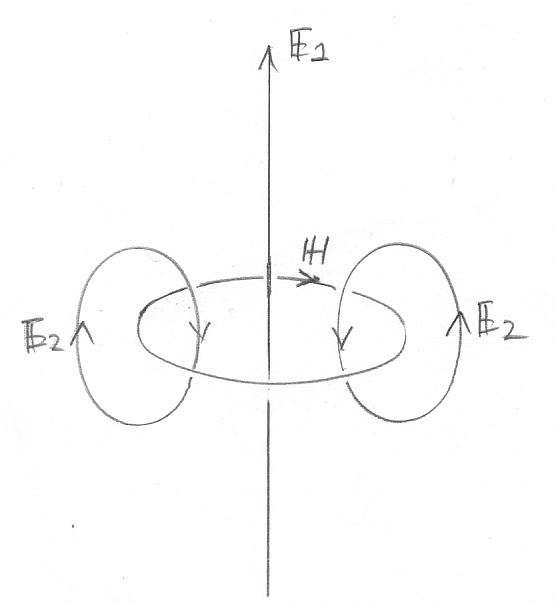
\includegraphics[width=0.4\textwidth]{IMG_20250411_0008.png}
  \caption{電磁波の概念}
  \label{abc}
\end{figure}

すると式(91)より、電界$\bm{E}$の周りに磁界$\bm{H}$が発生することがわかるので、$\bm{E_1}$の周りに磁界$\bm{H}$が発生する。
また、式(92)より磁界$\bm{H}$があればその周りに電界$\bm{E}$が発生することが分かるので、$\bm{E_1}$により発生した磁界$\bm{H}$はまたその周りに電界$\bm{E_2}$をつくる。

$\bm{E_2}$の$\bm{E_1}$側は$\bm{E_1}$を打ちけすような方向である。その分$\bm{E_2}$の外側は$\bm{E_1}$と同じである。これはすなわち、$\bm{E_1}$は$\bm{E_2}$となり垂直方向に広がったといえる。

\subsection{波動方程式}

式(91)にrotをとり、式(92)に代入すると、

\begin{align}
\mathrm{rot}\mathrm{rot}\bm{E}=-\mu\sigma\frac{\partial \bm{E}}{\partial t}-\mu\epsilon\frac{\partial ^2\bm{E}}{\partial t^2}
\end{align}

と、$\bm{H}$が消去される。媒質中に電荷がない場合($\mathrm{div}\bm{D}=\epsilon\mathrm{div}\bm{E}=0$)を考えると、ベクトル公式(A2.20)により

\begin{align}
\mathrm{rot}\mathrm{rot}\bm{E}=\mathrm{grad}\mathrm{div}\bm{E}-\bm{\nabla ^2-E}=\bm{-\nabla ^2E}
\end{align}

を得る。そのため式(93)は

\begin{align}
\mathrm{\nabla ^2E}=\mu\sigma\frac{\partial \bm{E}}{\partial t}+\mu\epsilon\frac{\partial ^2\bm{E}}{\partial t^2}
\end{align}

であり、これを\textbf{電磁波の波動方程式}という

\subsection{正弦波}

電界、磁界をそれぞれ正弦波

\begin{align}
\bm{E}=\sqrt{2}\bm{E'}e^{j\omega t},\bm{H}=\sqrt{2}\bm{H'}e^{j\omega t}
\end{align}

とする。これを式(91)、(92)に代入すれば、$\sqrt{2}e^{j\omega t}$で割ると

\begin{align}
\mathrm{rot}\bm{E'}=-\mu\cdot j\omega H' \\
\mathrm{rot}\bm{H'}=\sigma\bm{E'}+\epsilon\cdot j\omega\bm{E'}
\end{align}

を得て、ここで$\bm{E',H'}$を$\bm{E,H}$と書き直すと、

\begin{align}
  \mathrm{rot}\bm{E}=-\mu\cdot j\omega H \\
  \mathrm{rot}\bm{H}=\sigma\bm{E}+\epsilon\cdot j\omega\bm{E}
\end{align}

上式は式(91)、(92)の$\frac{\partial}{\partial t}$を$j\omega$に置き換えたものであるとわかる。
これが正弦波での特徴である。

ここで波動方程式(95)を

\begin{align}
k'^2=\omega ^2\epsilon\mu-j\omega\mu\sigma
\end{align}

とおけば、

\begin{align}
\nabla ^2\bm{E}+k'^2\bm{E}=0
\end{align}

と書くことができ、これを\textbf{ヘルツホルムの方程式}と呼ぶ。
また、回転をとれば

\begin{align}
  \nabla ^2\bm{H}+k'^2\bm{H}=0
  \end{align}

  である。

この式を便利に使うために直交座標系にとる。

\begin{align}
\begin{cases}
\frac{\partial E_z}{\partial y}-\frac{\partial E_y}{\partial z}=-j\omega H_x\\
\frac{\partial E_x}{\partial z}-\frac{\partial E_Z}{\partial x}=-j\omega H_y\\
\frac{\partial E_y}{\partial x}-\frac{\partial E_x}{\partial y}=-j\omega H_z \\
\end{cases}\\
\begin{cases}
\frac{\partial H_z}{\partial y}-\frac{\partial H_y}{\partial z}=(\sigma +j\omega\epsilon)E_x\\
\frac{\partial H_x}{\partial z}-\frac{\partial H_Z}{\partial x}=(\sigma +j\omega\epsilon)E_y\\
\frac{\partial H_y}{\partial x}-\frac{\partial H_x}{\partial y}=(\sigma +j\omega\epsilon)E_z
  \end{cases}
\end{align}

となり、マクスウェルの補足方程式は

\begin{align}
\frac{\partial E_x}{\partial x}+\frac{\partial E_y}{\partial y}+\frac{\partial E_z}{\partial z}=0\\
\frac{\partial H_x}{\partial x}+\frac{\partial H_y}{\partial y}+\frac{\partial H_z}{\partial z}=0
\end{align}

ヘルツホルムの方程式は

\begin{align}
\begin{cases}
\frac{\partial ^2E_x}{\partial x^2}+\frac{\partial ^2E_x}{\partial y^2}+\frac{\partial ^2E_x}{\partial z^2}+k^2E_x=0 \\
\frac{\partial ^2E_x}{\partial x^2}+\frac{\partial ^2E_x}{\partial y^2}+\frac{\partial ^2E_x}{\partial z^2}+k^2E_y=0 \\
\frac{\partial ^2E_x}{\partial x^2}+\frac{\partial ^2E_x}{\partial y^2}+\frac{\partial ^2E_x}{\partial z^2}+k^2E_z=0 
\end{cases}\\
\begin{cases}
  \frac{\partial ^2H_x}{\partial x^2}+\frac{\partial ^2H_x}{\partial y^2}+\frac{\partial ^2H_x}{\partial z^2}+k^2H_x=0 \\
  \frac{\partial ^2H_x}{\partial x^2}+\frac{\partial ^2H_x}{\partial y^2}+\frac{\partial ^2H_x}{\partial z^2}+k^2H_y=0 \\
  \frac{\partial ^2H_x}{\partial x^2}+\frac{\partial ^2H_x}{\partial y^2}+\frac{\partial ^2H_x}{\partial z^2}+k^2H_z=0 
  \end{cases}
\end{align}

ただし$k^2=\omega^2\epsilon\mu$である。

\subsection{平面波}

マクスウェル方程式の一番簡単な解をみていく。
そのため$\sigma=0$かつ、$\frac{\partial }{\partial x}=0,\frac{\partial}{\partial y}=0$とする。すると式(104),(105)より

\begin{align}
H_z=0,E_z=0
\end{align}

を得る。式(106),(107)は上式により自動的に満たされ、式(104)、式(105)より以下が残される。

\begin{align}
\frac{dE_x}{dz}=-j\omega\mu H_y,\frac{dH_y}{dz}=-j\omega\epsilon E_x\\
\frac{dE_y}{dz}=-j\omega\mu H_x,\frac{dH_x}{dz}=-j\omega\epsilon E_y
\end{align}

上記の二つの式はたがいに無関係であるので、独立して存在する。

\end{document}